%File: formatting-instruction.tex
\documentclass[letterpaper]{article}
\usepackage{aaai}
\usepackage{times}
\usepackage{helvet}
\usepackage{algorithm}
\usepackage{algpseudocode}
\usepackage{courier}
\usepackage{graphicx}
\graphicspath{{./figure/}}
\frenchspacing
\setlength{\pdfpagewidth}{8.5in}
\setlength{\pdfpageheight}{11in}
\pdfinfo{
/Title (Insert Your Title Here)
/Author (Put All Your Authors Here, Separated by Commas)}
\setcounter{secnumdepth}{0}  
 \begin{document}    

\section{Introduction}

Intelligent agents perceive the world mainly through images captured at different time points. The world keeps changing and most of the changes are spatial changes. e.g. changes in position, direction of the objects. A typical image captured by the agent is often composed of spatial objects and their relations. Their spatial properties and relations will change from one image to another. Those spatial changes are often resulted from objects motion.  Understanding those changes will help the agent to make sense of the world and perform meaningful tasks.

Object tracking, scene similarity, qualitative matching... 

Multiple objects tracking assumes objects' motions are independent and there are no interactions between the objects. Objects are often approximated. i.e. tracking  flights. A dynamic model is applied to estimate the motions of the targets.  

Another related problem is qualitative matching between two spatial scenes.\cite{}

Our problem is different from multiple target tracking because the objects in our case can interact and there is no well-defined dynamical model to estimate the objects motion.

Our problem is different from the qualitative spatial matching since the subsequent image may look totally different from the initial image regarding the spatial configurations. 


\section{Problem Description}
Finding the corresponding objects in next image can be formulated as a constraint satisfication problem (CSP), which consists of 
1) A set of variables corresponding to the objects in the initial image
2) A finite domain composed of the objects in the next image
3) One to one correspondence between the two sets is required

We use $o \sim o^{\prime}$ to denote a match between the spatial object $o$ and $o^{\prime}$. 
Given two object sets $O = \{o_1, o_2, ..., o_n\}$ and $O^\prime = \{o^{\prime}_{1}, o^{\prime}_{2}, ...., o^{\prime}_{m}\}$, a matching $M$ is bijection from $O$ to $O^\prime$.

Any matching $M$ between two scenes induces a series of spatial changes. A matching is admissible if the spatial change induced by the matching is achievable. [define achievable]. 

Some assumptions:
\begin{itemize}
\item Downwards gravity, continuous spatial change.
\item We know the time gap between two successive images
\item Only the objects of the same appearance can be matched. Objects appearance includes color, size and all other visual features. 
\item No new objects will be created in the subsequent image (except debris).
\item Initial image should not be crappy
\end{itemize}

Matching objects of different appearance is trivial, in the rest of paper, unless explicitly mentioned, the objects are supposed to be identical in terms of appearance and physical properties. We only consider rectangles and circles in 2 dimensional space. 

\section{Objects Representation with the extended GSR (EGSR)}

We use a minimum bounding rectangle to approximate the region occupied by a circle and use exact shapes for the rectangles.

The representation should allow us to infer possible motions of an object from its interaction with other objects. Since the objects can only interact via contacts, it is important to distinguish if and how two objects contact each other.  GSR is expressive enough to capture the contacts between a pair of solid rectangles. It defines eight contact sectors that correspond to the eight edges and corners of the rectangles. Given two GSRs $o_1$ and $o_2$ that contact each other via $sector_1, sector_2 \in \{S_1, ..., S_8, R_1, ..., R_8\}$, the contact relation between $o_1$ and $o_2$ can be expressed as the constraint $o_1 \, (sector_1, sector_2) \, o_2$. 

However, GSR introduces ambiguities when the rectangles are disconnected. To overcome the ambiguities, we partition the embedding space around the reference object into nine mutually exclusive tiles[cite, CDC]. The centre tile corresponds to the minimum bounding rectangle of the object and the other eight tiles correspond to the eight cardinal directions. 


Given two spatial objects, if the MBRs of the two objects intersect or boundary touch, we assign a GR relation accordingly. Otherwise, one of the eight cardinal tiles will be used to indicate the spatial relation. The GSR relation between a pair of objects can be obtained by first calculating the distance between each pair of the contact sectors and then using the sectors from the pair with the shortest distance. The distance becomes zero when the two objects touch. 

\begin{figure}[h!]
\centering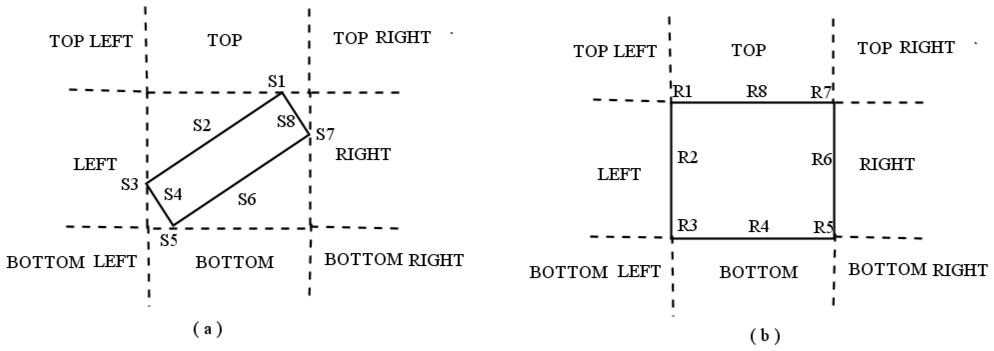
\includegraphics[scale=0.25]{EGSR-relations.png}\caption{Contact sectors and Cardinal directions of (a) an angular rectangle and (b) a normal rectangle}
\end{figure}

\section{Qualitative Motion Representation}

 To find out a best matching, a straightforward approach is to enumerate all the possible matchings. The search space is huge as there is a combinatorial number of matchings between two object sets. However, most of the matchings can be avoided by only searching through the corresponding objects in a limited area. The area of the initial object should therefore cover all the objects in the next scene that can be potentially matched to the initial object.  We use a circular region to represent such area. The circle centre is located at the centroid of the object and the radius of the circle is the maximum shift of the centroid. The radius is calculated by $V \times T$ where $V$ is the maximum velocity of the object while $T$ is the time gap. The calculation ensures the area estimation adaptable to different time gaps. We call this circle as $movement\,bounding\,circle$(MBC). 

The MBC can be divided into four quadrants to further restrict the search area. A quadrant is said to be open if all the objects in that quadrant can be considered as potential correspondence of the referred object, otherwise the quadrant is closed.  

 Given a MBC $C$, if we want to explicitly talk about the quadrants that are open, we write $C^{(i,j)}, (i,j) \in \{-, +, *\}$ wrt. the given MBC, where $(+,+)$, $(+,-)$, $(-,-)$, $(-,+)$ correspond to the top-right, top-left, bottom-left, bottom-right quadrant respectively. $(*, *)$ refers to an arbitrary quadrant. 
\begin{figure}[h!]
\centering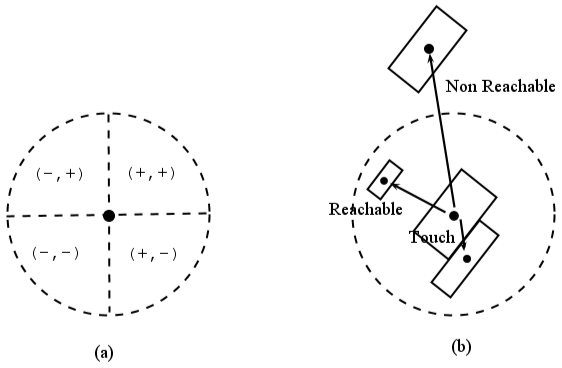
\includegraphics[scale=0.3]{quadrants.png}\caption{(a) The four quadrants of a MBC (b) Qualitative distance with respect to object A and its MBC}
\end{figure}
By estimating the movement direction of the object, we can infer the open quadrants by estimating which of the quadrants the object is most likely to be in at the next time point. The initial object will then be matched with one of the objects within the open quadrants while outside objects will not be considered.

Movement direction can be approximated by analysing the structural properties, e.g. the stability of an object. An object is stable when it is supported and remains static. When an object is not stable, there will be two possible motions: 1) free fall if it has no supports. 2) fall to the side where supports are absent. 

\cite{Ge2013} proposed four kinds of supports that can make a solid rectangle stable. We utilize these stable configurations and estimate the open quadrants accordingly. E.g. given an object supported by one edge support, if the right side support is removed, then it is likely to fall to right, thus the open quadrant is $C^{(+,-)}$
(see Figure \ref{QudrantsEstimation}). 

\begin{figure}[h!]\label{QudrantsEstimation}
\centering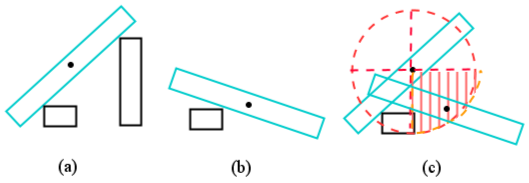
\includegraphics[scale=0.4]{QudrantsEstimation.png}\caption{(a) the object in cyan is supported via one-edge support  (b) a subsequent scene after the right support is removed (c) The estimated open quadrant (shadowed area) approximates the subsequent centroid location}
\end{figure}

Now we can distinguish the relative distance between two objects into three meaningful classes, namely touch, reachable, and non reachable. An object $O$ can touch another object $O^\prime$ by one of its contact sectors. $O^\prime$ is reachable to $O$ if $O^\prime$ is within the MBC of $O$ otherwise non reachable.



\section{Tracking by spatial reasoning}\label{trackingBySpatialReasoning}

One challenge is to find out a matching between identical objects that are close to each other, and have the similar motions.  
\begin{figure}[h!]\label{SCOExample_2}
\centering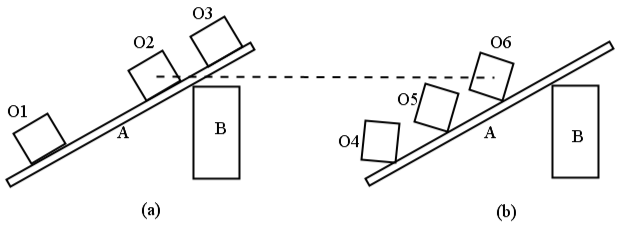
\includegraphics[scale=0.3]{SCOScenario_2.png}\caption{(a) an initial scene (b) a subsequent scene}
\end{figure}
Figure \ref{SCOExample_2}.a  shows a scene where object A and B forms a slope and there are three identical squares $O_1$, $O_2$ and $O_3$ lying on the slope. Figure \ref{}.b is a subsequent image where the three squares went down a bit. There are 6 ways to match between the squares while only $\{O_1 \sim O_4, O_2 \sim O_5, O_3 \sim O_6\}$ is possible. Without reasoning about the spatial relations between the squares, some optimization algorithms, e.g. minimizing centroid shift, will tend to match $O_2$ with $O_6$. In many cases, objects dynamics such as velocities are unavailable, thus most of state of the art tracking algorithms do not apply well because of the lack of a suitable dynamic model. 

Human can solve this case efficiently by spatial reasoning. Since we know the objects are moving at the similar velocity, the relative spatial changes among them can be subtle. Hence the spatial relations between those objects can hardly change to the opposite abruptly as they are moving. When matching, we are trying to keep the original spatial relations among the objects. 

We propose a method to deal with this in two steps, 1) identify those objects that will follow the similar motion 2) applying spatial constraints check on those objects when evaluating a match. 


We assume that the objects are likely to follow a common motion if they have the same contact relations with the same objects. We call the group of objects that are likely to share a common motion as $spatially\,\,correlated\,\,objects$ (SCO). Figure \ref{SCOExample} shows some examples of SCO in a typical angry birds scenario. 
\begin{figure}[h!]\label{SCOExample}
\centering\includegraphics[scale=0.7]{SCOScenario.png}\caption{(a) A typical angry birds scenario (b) the corresponding SCOs (highlighted by different color)}
\end{figure}
By finding groups of such objects we can then apply the spatial constraints among them when evaluating a match. 

Formally, let $R$ be a set of EGSR relations and $oppo(r), r\in R$ be the opposite set of relations of $r$. Given a group of spatially correlated objects in the initial image $O = \{o_1, o_2, ... , o_k\}$, and a set of objects in the next image $O^\prime = \{o^{\prime}_1, o^{\prime}_2, ..., o^{\prime}_k \}$ where $o_i \sim o^{\prime}_i, i \leq k$, $\exists r\in R\,\, o_i \{r\} o_j \Rightarrow \forall r^{\prime} \in oppo(r)\,\, o^{\prime}_i \{r^{\prime}\} o^{\prime}_j $ does not hold. In the slope example, a match $\{O_1 \sim O_4, O_3 \sim O_5, O_2 \sim O_6\}$ violates the constraint because $O_2 LEFT O_3$, $O_6 RIGHT O_5$ and $RIGHT \in oppo(LEFT)$  

 [list opposite set for each relation]


\section{A method for Objects Tracking}l disappear. The debris can be of 
We applied all the techniques mentioned above to solve the problem in the 

Let $O$ and $O^{\prime}$ be a set of objects in an initial image and a subsequent image taken at a later time, respectively. For ease of notation, we will refer to objects in $O$ as initial objects and objects in $O^{\prime}$ as new objects.

First, the method randomly assigns a unique ID to each initial object, and estimates the MBC quadrants of each object according to the object's spatial relations. The domain for each initial object is set so that it contains only the new objects that are of the same object type and within the MBC quadrants. The method then creates a preference list from the domain of each of the initial objects: the new objects in the preference list are sorted by the size of the centroid shift from the initial object in ascending order. The method matches the two sets of objects using a stable marriage algorithm with the pre-computed preference lists. The algorithm ensures each match is stable in the sense that no pair of objects would prefer each other over their matched partners. 

Then, the method finds all groups of spatially correlated objects among the initial objects and gets their corresponding objects from the match. The method then checks to see whether a spatial constraint has been violated, as mentioned in \ref{trackingBySpatialReasoning}. If there has, it resolves it accordingly.


\section{Evaluation}
 We implemented our method and applied it to the Angry Birds where the vision can detect the exact shapes of the objects\cite{}. For each detected object, the vision assigns a type according to the object's color, the main types are $stone, wood, ice$. The vision has the following limitations: 1) Damaged objects will be detected as a few separate smaller objects. 2) Debris are not recognized so that one cannot determine whether an object of type stone is a real stone or just a piece from a previously destroyed stone. 3) Objects occlusion is not handled.  We show those problem can be dealt with effectively by the above mentioned techniques. 

 \section{Debris Recognition}
Destruction of an object will create a cluster of debris around the object's location. Those debris can be of any shape, e.g. circle, polygon and will spread until disappear after 2-4 seconds. We can infer the destruction of a certain object by recognizing the 
he debris can not be recognized 
\section{Damage Status Recognition}


\section{Object Occlusion Management}  




\section{Obtaining Ground Truth}
 We capture a sequence of images before and after a shot. 
We first evaluate our method on a sequence of images captured with the smallest time gaps(50 ms). The resulting matchings are recorded and set as ground truth in the later evaluations. 

We evaluate our method by varying the time gaps.




\begin{algorithm}[!]
\caption{The Object Tracking Algorithm}\label{algo}
\begin{algorithmic}[1]
\Procedure {MatchObjects}{$objs$}
\State $iniobjs$ //initial objects
\State $solution \leftarrow \{iniobjs, \{\}\}$
\State $domain \leftarrow \{\}$// A map stores each initial object and a list of possible correspondence 
\State $domain \leftarrow$ MotionEstimation($objs$) 
\State CalculatePreference($iniobjs$, $domain$) //Calculate the preference list of $iniobjs$
\State $freeobjs \leftarrow iniobjs$
\While{$freeobjs$ is not empty}
\State $iniobj \leftarrow freeobjs.pop()$
\State get a next preferred $obj$ from $iniobj$'s preference list  
\If {$obj$ is not assigned yet}
  \State match($iniobj$, $obj$)
  \Else{$obj$ has been assigned to $iniobj^{\prime}$}
  \If{$obj$ prefers $iniobj$ to $iniobj^{\prime}$}
  \State match($iniobj$, $obj$), add $iniobj^{\prime}$ to $freeobjs$
\EndIf 
\EndIf
\EndWhile
\State $cobjsList \leftarrow$ GetSCO($objs$)// get spatially correlated objects
\State SPC($solution$) //Spatial Constraints Check
\State $iniobjs \leftarrow objs$
\EndProcedure

\Procedure{GetSCO}{$objs$}
\State $cobjsList \leftarrow \{\}$
\For {$obj \in objs$}
\State $cobjs \leftarrow objs$ 
\State $tobjs \leftarrow$ a set of the objects that touch $obj$
\For {$tobj \in tobjs$}
\State $ttobjs \leftarrow$ a set of the objects excluding $obj$ that touch $tobj$ via the same contact relation.
\State $cobjs \leftarrow cobjs \cap ttobjs$
\EndFor
\State $cobjsList \leftarrow cobjsList \cup cobjs$
\EndFor
\Return $cobjsList$
\EndProcedure
\Procedure{MotionEsimation}{$objs$}
\For {$obj \in objs$}
\State $domain \leftarrow domain \cup \{obj, \{\}\}$
\State $pobjs \leftarrow \{\}$
\State compute the MBC of $obj$
\State analyse the stability of $obj$ according the rules specified in \ref{} and locate the corresponding quadrants.
\State Remove the objects which are of different type, and add the remaining objects in the quadrants to $pobjs$. 
\State $domain \leftarrow domain \cup \{obj, \{pobjs\}\}$
\EndFor
\Return $domain$
\EndProcedure
\Procedure{Match}{$iniobj$, $obj$}
\State $obj.id \leftarrow iniobj.id$, $solution \leftarrow \{iniobj, obj\}$
\EndProcedure
\Procedure{SPC}{$solution$}
\For {$cobjs \in cobjsList$}
\State for each object in $cobjs$, get its matched $obj$ from $solution$
\State Check whether the spatial constraints \ref{} are violated. If violated, re-assign the objects until violation is resolved  
\EndFor
\EndProcedure
\end{algorithmic}
\end{algorithm}
 \end{document}